\section*{Introduction}

\begin{frame}{\ttfamily ./whoami}
  \begin{columns}
    \column{0.75\textwidth}
    \begin{description}
        \setlength{\itemsep}{2ex}
      \item[2024--\textit{now}\hfill] Postdoc, University of Luxembourg, SnT, Luxembourg\\
        {\small\color{gray}
          \alert{Security} and \alert{monitoring} of locally distributed systems.\\
        With \textexample{Jérôme François}, academic (COCTEL, FNR) and industrial (PAIGE, Thales Luxembourg) projects.}
      \item[2020--2024\hfill] PhD, IMT Atlantique, IRISA/SOTERN, Rennes\\
        {\small\color{gray} "Improving \alert{intrusion detection} in distributed systems with \alert{federated learning}"\\
          Supervised by \textexample{Yann Busnel}, co-supervised by \textexample{Fabien Autrel} and \textexample{Marc-Olivier Pahl}, industrial funding (Chair CyberCNI).\\
        \textbf{GDR RSD PhD Thesis Award, 2025}.}
      \item[2017--2020\hfill] Eng. Degree in Information Security, ENSIBS, Vannes\\
        {\small\color{gray} Part-time employee at Orange Cyberdefense, Rennes, \alert{application security} and DevSecOps.}
    \end{description}

    \column{0.30\textwidth}
    \centering
    \includegraphics[width=.9\linewidth]{figures/lavaur_snt.png}
    \vspace{1em}

    Intrusion Detection\\
    Federated Learning\\
    Security of AI Systems\\
    Network/System Security\\

  \end{columns}

  \begin{minipage}{0.85\textwidth}
  \end{minipage}
\end{frame}

\begin{frame}[t]{Intrusion Detection in Organizations}

  \begin{columns}
    \column{0.55\textwidth}
    \begin{block}{Intrusion detection system (IDS)}
      Automated tool for identifying \alert{malicious} activity
    \end{block}

    \onslide<3->{%
      \begin{block}{Solved\only<4>{{\usebeamercolor{alerted text}\color{fg}\footnotemark}} thanks to machine learning!}
        99\% accuracy on public benchmarks
    \end{block}}

    \column{0.45\textwidth}
    \centering%
    \includegraphics<1>[width=1.1\textwidth,center]{figures/intro/ids-1.pdf}%
    \includegraphics<2>[width=1.1\textwidth,center]{figures/intro/ids-2.pdf}%
    \includegraphics<3->[width=1.1\textwidth,center]{figures/intro/ids-3.pdf}%
  \end{columns}

  \only<4>{\footnotetext{Assuming high-quality datasets that are representative of real-world scenarios\dots}}
\end{frame}

% \begin{frame}[t]{Collaboration and Federated Learning}
%   \setbeamercolor{itemize item}{fg=example text.fg}\vspace{-1em}
%   \vspace{1em}
%   \begin{columns}
%     \column{0.5\textwidth}
%     \begin{itemize}[<+->]
%         \setlength{\itemsep}{1ex}
%       \item Similar tasks in numerous organizations
%       \item Towards collaborative approaches?
%       \item Data too sensitive to be shared
%       \item Solution: \alert{federated learning} (FL)
%     \end{itemize}

%     \column{0.5\textwidth}
%     \centering
%     \foreach \i in {1,...,3} {\includegraphics<\i>[width=1.1\textwidth,center]{figures/intro/cids-\i.pdf}}%
%     \includegraphics<4->[width=1.1\textwidth,center]{figures/intro/fids.pdf}%

%   \end{columns}

%   \onslide
%   \begin{center}
%     {\large\bfseries Can \alert{FL} serve as a \alert{collaboration} tool for intrusion detection?}
%   \end{center}
% \end{frame}

\begin{frame}[t]{A Distributed Problem}
  \begin{columns}
    \column{0.5\textwidth}
    \begin{block}{Similar tasks in numerous organizations}
      Different attacks and devices but same challenge
    \end{block}

    \onslide<2->{%
      \begin{block}{Incentives to collaborate}
        \begin{itemize}
          \item common interest (\eg, inter-SOCs\only<2>{\footnotemark})
          \item national agencies (\eg, NIST, ANSSI)
          \item regulation (\eg, private-public information sharing in NIS2)
        \end{itemize}
    \end{block}}

    \column{0.5\textwidth}
    \centering
    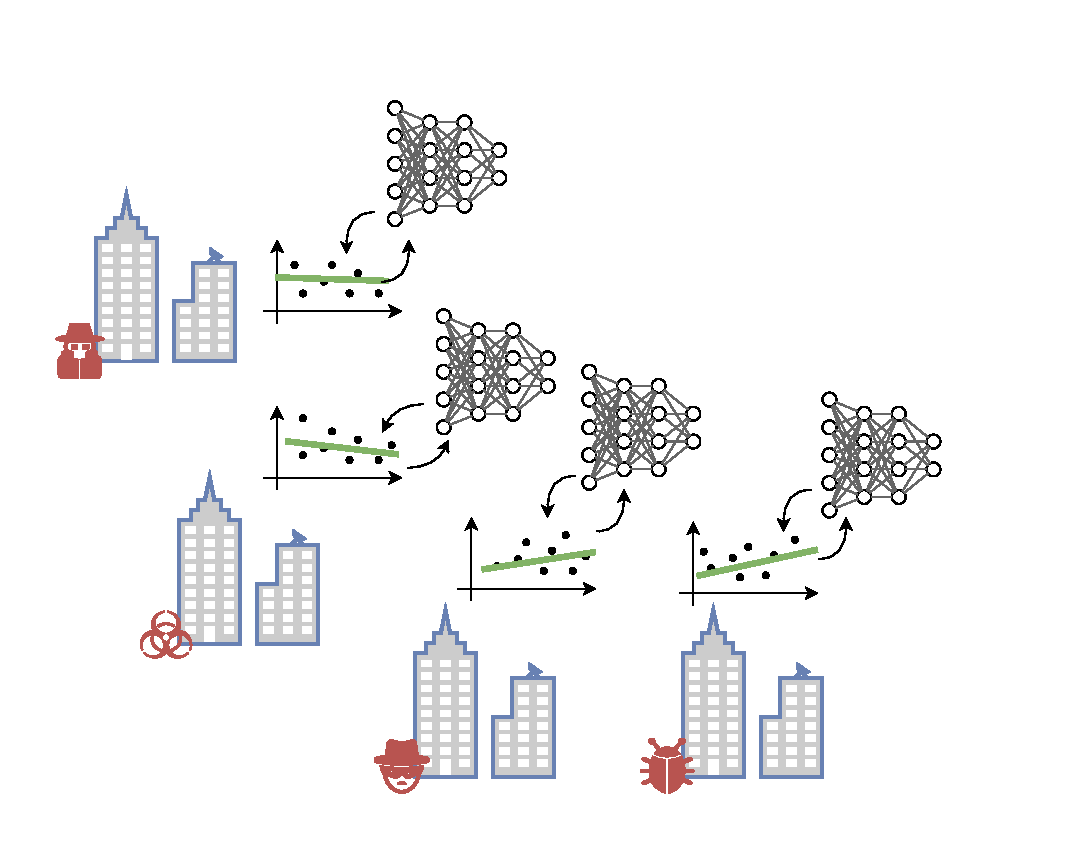
\includegraphics[width=1.1\textwidth,center]{figures/intro/cids-1.pdf}%
  \end{columns}

  \only<2->{\footnotetext{Security Operations Centers.}}
\end{frame}

\begin{frame}[t]{Collaborative Learning}
  \begin{columns}
    \column{0.5\textwidth}

    \textbf{Let's pool our data!}\onslide<2->{
      \textbf{Although\dots}

      \begin{itemize}
        \item Privacy concerns.
        \item Lack of trust in the data holder.
        \item Lack of trust in the learning process.
        \item \dots
    \end{itemize}}

    \column{0.5\textwidth}
    \centering
    \includegraphics<1>[width=1.1\textwidth,center]{figures/intro/cids-2.pdf}%
    \includegraphics<2->[width=1.1\textwidth,center]{figures/intro/cids-3.pdf}%
  \end{columns}
\end{frame}

\begin{frame}[t]{Federated Learning}
  \begin{columns}
    \column{0.5\textwidth}
    \textbf{The solution: \alert{Federated Learning} (FL)}~\autocite{mcmahan_Communicationefficientlearningdeep_2017}
    \begin{itemize}
      \item Clients train a common model without sharing data
      \item Only model updates are shared with a central server
      \item More privacy-friendly
    \end{itemize}
    \column{0.5\textwidth}
    \centering
    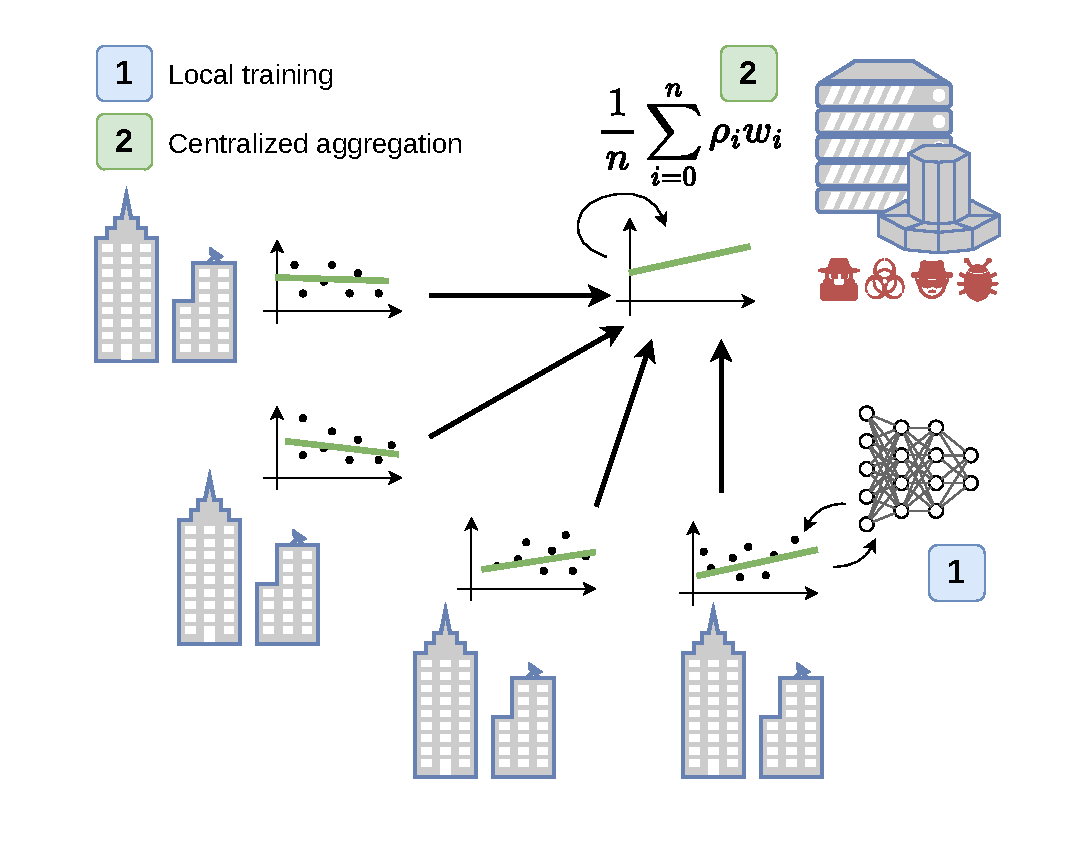
\includegraphics[width=1.1\textwidth,center]{figures/intro/fids.pdf}%
  \end{columns}
  \pause
  \only<1>{\footcite*{mcmahan_Communicationefficientlearningdeep_2017}}
  \only<2->{
    \begin{center}
      {\large\bfseries Can \alert{FL} serve as a \alert{collaboration} tool for intrusion detection?}
    \end{center}
  }
\end{frame}